\chapter{Einleitung}\label{Einleitung}
Obwohl es bereits zahlreiche Wege gibt, um Input eines Nutzers in die virtuelle Realität zu übersetzen, sind die Möglichkeiten für Feedback zurück in die reale Welt hingegen spärlich. Haptischer Feedback ist in diesem Kontext ein Oberbegriff für solche Möglichkeiten, die einem Nutzer das Gefühl seines Avatars aus der virtuellen Realität zu übermitteln versuchen. Es existieren bereits einige Konzepte für haptischen Feedback, wie zum Beispiel Vibration, Bewegungseinschränkung (Force-Feedback) und Simulation von Gewicht/Textur. Allerdings ist die Umsetzung dieser Konzepte in tatsächlichen Geräten durchaus problematisch, da sich ein normaler Endnutzer in der Regel zwischen zufriedenstellender Funktionalität und einem erschwinglichen Preis entscheiden muss.\\
Xaiochi Gu et al. haben versucht, dieses Problem zu lösen. Als Mechanical and Control Engineering Student in Cambridge hat Gu für seine Abschlussarbeit Dexmo entwickelt: ein Exoskelett, das sich größtenteils auf dem Handrücken des Nutzers befindet und durch Motion Capturing und Force-Feedback ein verbessertes Erlebnis in der virtuellen Realität herbeiführen kann. Dexmo wurde in den ''Proceedings of the 2016 CHI Conference on Human Factors in Computing Systems'' publiziert und Gu arbeitet seit dem Ende seines Studiums als CEO von Dextra Robotics an weiteren Iterationen von Dexmo. 

\begin{figure}[!ht] % see https://en.wikibooks.org/wiki/LaTeX/Floats,_Figures_and_Captions for placement parameters
\centering

\includegraphics[width=0.4\textwidth]{images/xiaochi.png}
\caption{Xaiochi Gu}
\end{figure}


\chapter{Hintergrund}\label{Hintergrund}

In der Vergangenheit wurden bereits einige Versuche unternommen, Geräte mit Force-Feedback für die Hände umzusetzen. Eines solcher Geräte ist PHANTOM; ein Schreibstift, der an einem mechanischen Arm befestigt ist. Nutzer können mit dem Stift in der virtuellen Realität schreiben und zeichnen, wobei der mechanische Arm die Bewegung einschränkt, sobald die virtuelle Repräsentation des Stiftes auf ein Hindernis stößt. PHANTOM funktioniert präzise, aber hat nur einen limitierten Anwendungsbereich, da es auf Interaktion mit virtuellen Stiften beschränkt ist.
\begin{figure}[!ht] % see https://en.wikibooks.org/wiki/LaTeX/Floats,_Figures_and_Captions for placement parameters
\centering
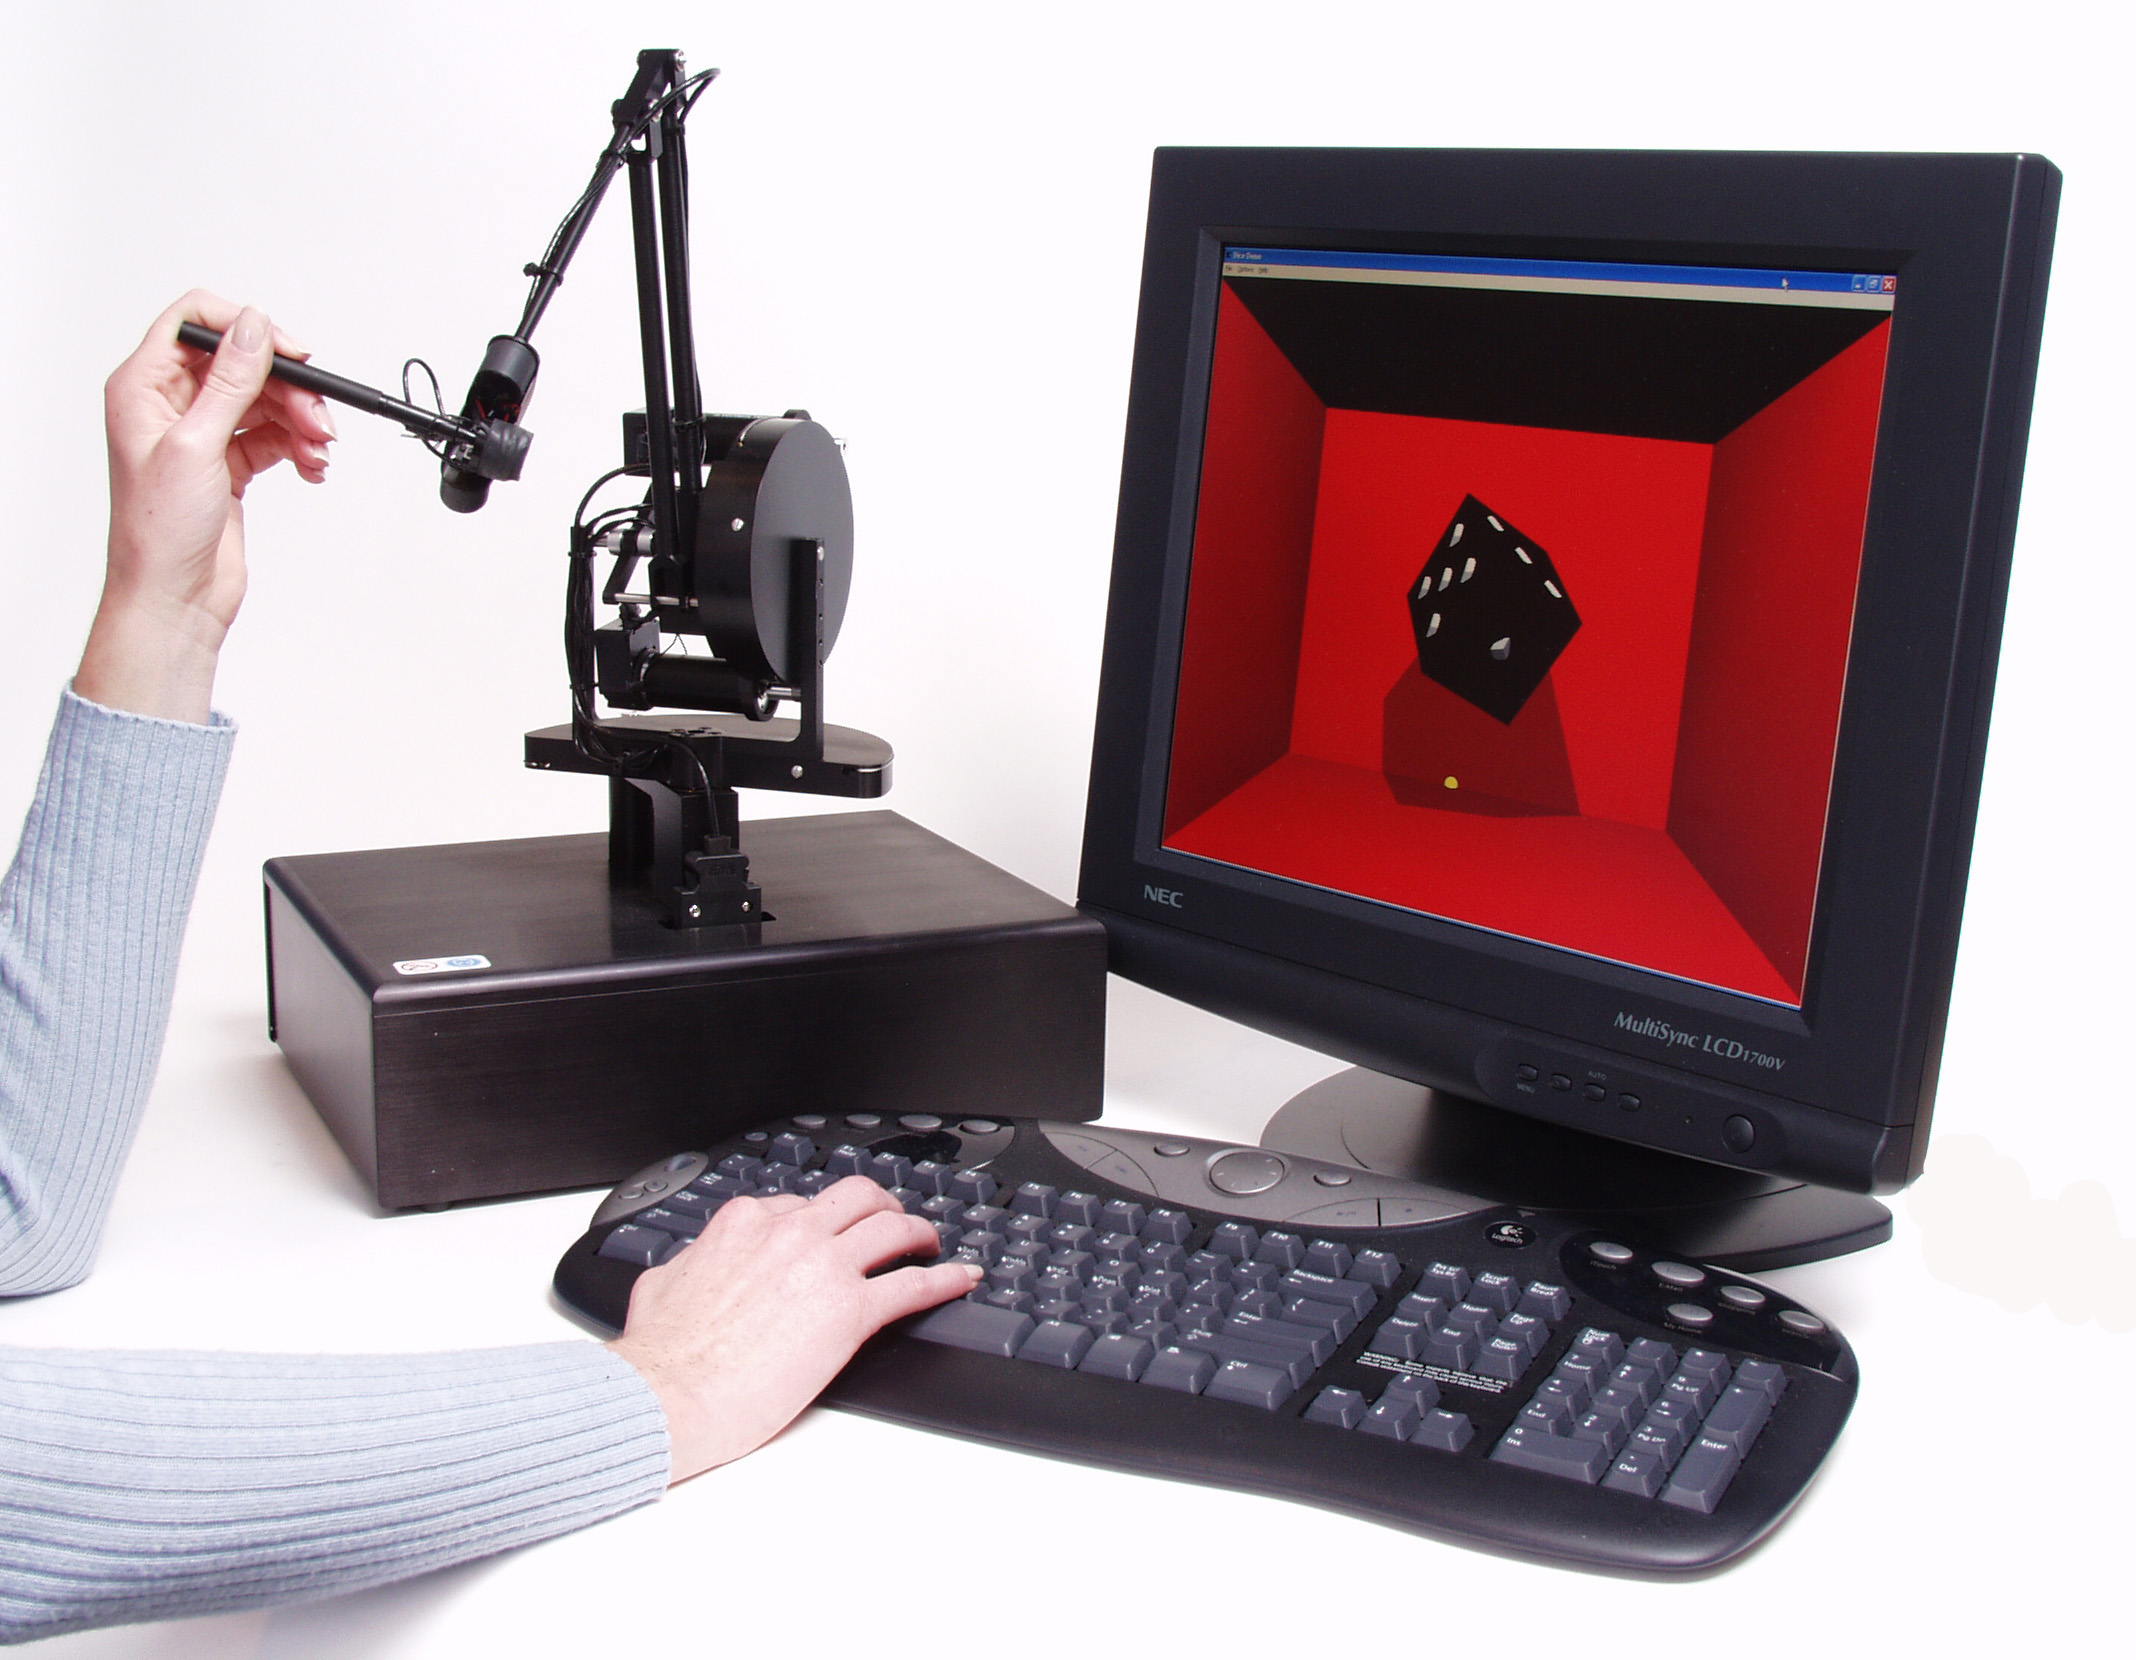
\includegraphics[width=0.2\textwidth]{images/Phantom.jpg}
\caption{PHANTOM}
\end{figure}

Ein weiterer Versuch ist der Rutgers Master II-ND; ein Handschuh, dessen Force-Feedback durch ein Konstrukt auf der Innenfläche der Hand realisiert wird. Dieses Gerät hat einen weitaus größeren Anwendungsbereich als PHANTOM, aber es schränkt die Bewegungsfreiheit von Nutzern ein, da es unmöglich wird, ihre Hand komplett zu einer Faust zu schließen. Des Weiteren sorgt eine komplexe Force-Feedback-Einheit für den hohen Preis des Gerätes.

\begin{figure}[!ht] % see https://en.wikibooks.org/wiki/LaTeX/Floats,_Figures_and_Captions for placement parameters
\centering
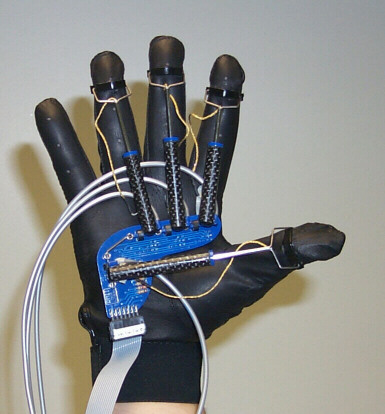
\includegraphics[width=0.2\textwidth]{images/Rutgers.jpg}
\caption{Rutgers Master II-ND}
\end{figure}


\chapter{System Design}\label{System Design}

Dexmo besteht aus folgenden Komponenten; Force-Feedback-Einheiten, Konnektoren, Fingerkappen und einem Main-Controller. Die Fingerkappen werden an den einzelnen Fingern eines Nutzers befestigt, während der Main-Controller auf dem Handrücken sitzt. Die Konnektoren verbinden die einzelnen Kappen mit dem Main-Kontroller, wobei sich zusätzlich fünf Force-Feedback-Einheiten zwischen dem Main-Kontroller und den jeweiligen Fingerkappen befinden. Der Main Kontroller sendet Motion Capturing Informationen von allen Sensoren an einen angeschlossenen Computer und gibt außerdem den Befehl für Force-Feedback, falls der Computer seinerseits eine Kollision in der virtuellen Realität erkennt.

\begin{figure}[!ht] % see https://en.wikibooks.org/wiki/LaTeX/Floats,_Figures_and_Captions for placement parameters
\centering
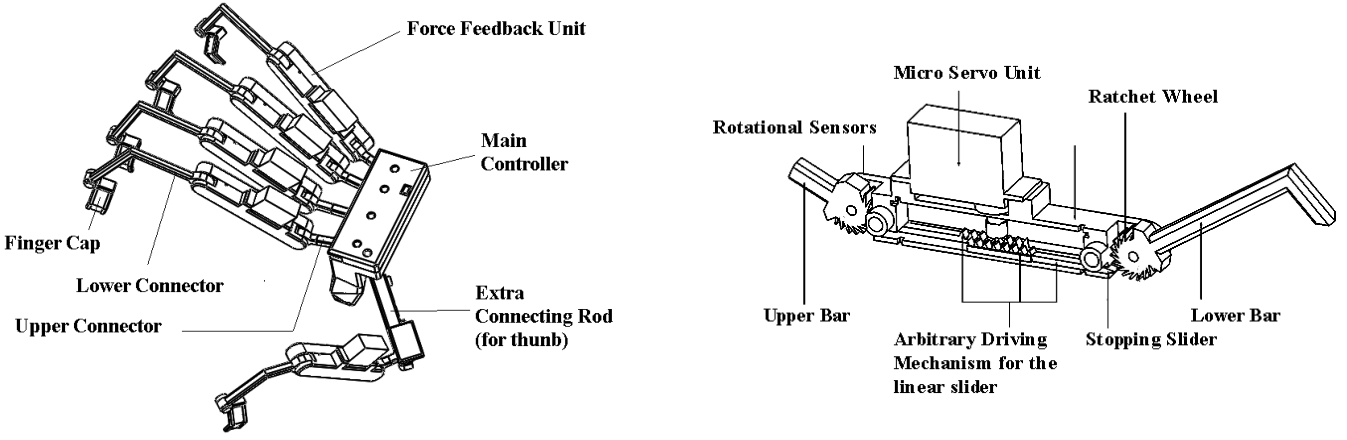
\includegraphics[width=0.8\textwidth]{images/dexmo-structure.png}
\caption{Das mechanische Design von Dexmo}
\end{figure}

Der wichtigste Teil des Designs ist die Force-Feedback-Einheit, weil hier das geringe Gewicht und der niedrige Preis von Dexmo realisiert werden. An den Zahnrädern, die für die Beweglichkeit im Normalzustand sorgen, befinden sich Rotationssensoren. Diese Sensoren erkennen wann und wie sehr sich ein Zahnrad bewegt und können dadurch die Informationen über Fingerbewegung an den Main-Controller weitergeben. Sobald eine solche Fingerbewegung für eine Kollision in der virtuellen Realität sorgt, gibt der Main-Controller den Force-Feedback-Befehl an die relevanten Force-Feedback-Einheiten zurück. Daraufhin blockieren Schieberegler in den Einheiten die Zahnräder und schränken dadurch die Bewegung des Nutzers ein. Diese Blockade gibt Nutzern den Eindruck, dass sich etwas in dessen Hand befindet. Dank dieser Implementation muss keine echte Kraft auf Nutzer ausgeübt werden, wodurch Dexmo zusätzlich auch sicherer als vergleichbare Produkte geworden ist. Außerdem gibt es keine designbedingte Einschränkung der Motion Capturing-Funktionalität, da keine Komponente die Innenseite einer Hand blokiert. 

\chapter{Design Trade-Offs}\label{Design Trade-Offs}
Dexmo benötigt dank seiner Kompaktheit und des geringen Gewichtes keinen kabelgebundene Stromversorgung. Eine normale 800mAh Batterie leistet bereits 4 Stunden Laufzeit. Andere kommerzielle Geräte wie Cybergrasp benötigten weitaus mehr Energie für gleichwertige Funktionalität. Des Weiteren sorgt das modulare Design und der Verzicht auf teure Motoren für geringe Manufakturkosten. Ein einzelner Motor von einem high-end Gerät kann in der Regel mehr kosten als alle von Dexmo benötigten Materialien zusammen. Zusätzlich sorgt das modulare Design auch für eine erhöhte Robustheit des Gerätes, da alle Kleinteile von ihren Gehäusen umschlossen sind und keine freiliegenden Sehnen für die Gelenke gebraucht wurden.\\
Allerdings gibt es auch einige Nachteile am Design von Dexmo; Momentan ist nur binärer Force-Feedback möglich, weshalb man die Nachgiebigkeit eines Objektes in der virtuellen Realität nicht simulieren kann. Nur die Form eines Objektes kann von Dexmo dargestellt werden, indem lediglich einzelne der fünf Force-Feedback-Einheiten blockiert werden. Außerdem sorgen die Schiebemechanismen für eine Verzögerung von 20-40ms. Für eine immersive Nutzererfahrung ist es in der Regel nötig, die Verzögerung auf 30ms beschränken zu können.

\begin{figure}[!ht] % see https://en.wikibooks.org/wiki/LaTeX/Floats,_Figures_and_Captions for placement parameters
\centering
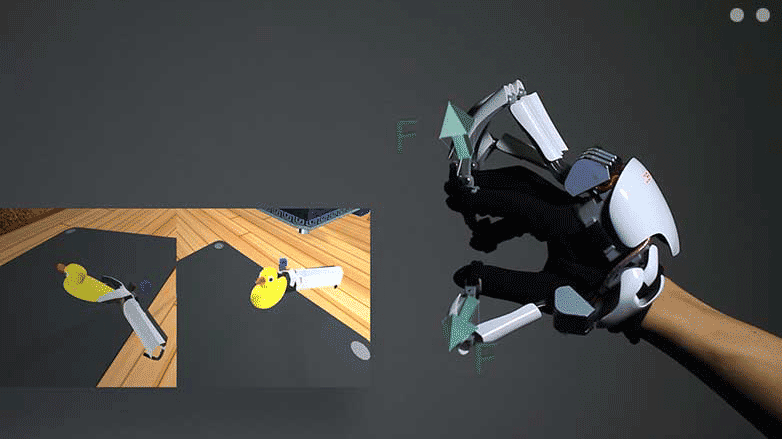
\includegraphics[width=0.8\textwidth]{images/concept.png}
\caption{Konzept für eine neue Iteration von Dexmo mit Force-Feedback für Nachgiebigkeit}
\end{figure}

\chapter{Evaluation und Ergebnisse}\label{Evaluation und Ergebnisse}

Die Effizienz des Gerätes wurde in einem informellen Labortest verifiziert. Das Ziel dieser Studie war die Validierung, dass Dexmo von typischen Endnutzern für simple Aufgaben in der virtuellen Realität problemlos benutzt werden kann. Dazu wurden 20 Teilnehmer aus diversen Bereichen herangezogen. Hierbei handelte es sich insgesamt um Studenten, Athleten, Ingenieure, Putzkräfte, Spieleentwickler und Fabrikarbeiter. Unter den Probanden waren zehn Frauen und zehn Männer.\\
Um die Funktionalität von Dexmo zu testen, wurde ein spielerisches Szenario entwickelt; Die Probanden mussten in der virtuellen Realität Pfeile aufheben, sie in einen Bogen setzen, die Bogensehne spannen und schlussendlich auf ein Ziel schießen. Dabei wollten Gu et al. herausfinden, welchen Einfluss Force-Feedback auf die Fehlerrate beim Zielen hat. Ihre Null-Hypothese: Force-Feedback sorgt für keine signifikante Änderung in der Fehlerrate.\\
Um diese These zu wiederlegen, wurde im Labortest eine unabhängige Variable mit zwei Level benutzt und within-subject Design angewandt: Zuerst schießen die Probanden 10 Pfeile mit Force-Feedback. Nach einer einstündigen Pause wurde das Experiment ohne Force-Feedback wiederholt. Für diese Studie war aus drei Gründen kein Counterbalancing nötig: Erstens war das Szenario so simpel, dass ein Lerneffekt als unerheblich bezeichnet wurde. Zweitens sorgt die einstündige Pause dafür, dass Muscle Memory kein Faktor ist. Und drittens besagt die Null-Hypothese, dass Force-Feedback keinen Einfluss auf die Fehlerrate hat, wodurch Gu et al. davon ausgehen können, dass der zweite Testdurchlauf bei einer wahren Null-Hypothese auf jeden Fall keine signifikant höhere Fehlerrate aufweisen darf. \\
Nach Abschluss der Studie hat sich gezeigt, dass die Fehlerrate mit Force-Feedback noch bei 44\% lag und ohne Force-Feedback auf 61\% angestiegen ist. Bei einem Signifikanzlevel von $\alpha = 0.05$ ist diese erhöhte Fehlerrate statistisch signifikant. Die Kombination von geringem p-Wert und hoher Effektgröße deutet außerdem darauf hin, dass die entdeckte Differenz robust und erheblich ist. Damit hat sich gezeigt, dass Force-Feedback einen positiven Effekt auf Performance in der virtuellen Realität hat. 

\chapter{Diskussion und Schlussfolgerung}\label{Diskussion und Schlussfolgerung}

In dieser schriftlichen Ausarbeitung wurde Dexmo vorgestellt: ein mechanisches Exoskelett von Gu et al. für Force-Feedback und Motion Capturing in der virtuellen Realität. Im Vergleich zu anderen Force-Feedback Geräten bietet Dexmo nur binären Feedback, aber hebt sich trotzdem durch ein innovatives Design von der Konkurrenz ab. Durch Schiebemechanismen konnten bei Dexmo auf teure Sensoren und sperrige Motoren verzichtet werden, wodurch ein leichtes und handliches Gerät entstanden ist, das sich für den Massenverbrauchermarkt bestens eignet. Außerdem sorgt der modulare Aufbau für ein robustes Produkt und der Energieverbrauch ist ebenfalls vergleichsweise gering. \\
Des Weiteren konnte die Funktionalität von Dexmo in einer Studie validiert werden. Durch ein spielerisches Laborexperiment wurde sowohl die zuverlässige Arbeitsweise als auch eine verringerte Fehlerrate von Probanden festgestellt, solange Dexmos Force-Feedback ausgenutzt wurde. Die informellen Eindrücke dieser Probanden waren ebenfalls durchweg positiv.

%%%%%%%%%%%%%%%%%%%%%%%%%%%%%%%%%%%%%%%%%%%%%



% keep an blank line above

